\documentclass[../main.tex]{subfiles}

\begin{document}
\chapter{Drivers of Antarctic Land Ice}
\label{chap:land_ice}
In chapter \ref{chap:temp_and_ice}, we found that temperature is significant for our understanding of the trends in Antarctic \gls{sic} over the last 40 years. However we found that the relationship between temperature and land ice is not as strong. To understand this we will have to do some more calculations.

We want to consider a range of variables which could be impacting land ice in Antarctica. We will include temperature again for completeness. Wind speed is linked to atmospheric circulations which move clouds and thermal energy around the continent. Cloud cover has also been linked to behaviours in the land ice. \textcolor{red}{add appropriate citations here}. 

\section{Time-frame of datasets used in this chapter}
For this chapter we use a number of datasets, which each have data available for different time frames. Because of the limitations in table \ref{tab:landicedata} we will restrict our time-frame to 2014 - 2017.
% Please add the following required packages to your document preamble:
% \usepackage{booktabs}
\begin{table}[H]
\begin{tabular}{@{}lll@{}}
\toprule
Data                                     & Start Date   & End Date \\ \midrule
ECMWF ERA5 Reanalysis                    & January 1981 & Present  \\
GRACE \gls{LILWET}                       & August 2002  & 2017  \\
ARGO product \textcolor{red}{check this} & January 2004 & Present  \\ \bottomrule
\end{tabular}
\caption{Different data sources used in this chapter.}
\label{tab:landicedata}
\end{table}

\section{Land ice trends and variability}
 \begin{figure}[H]
     \centering
     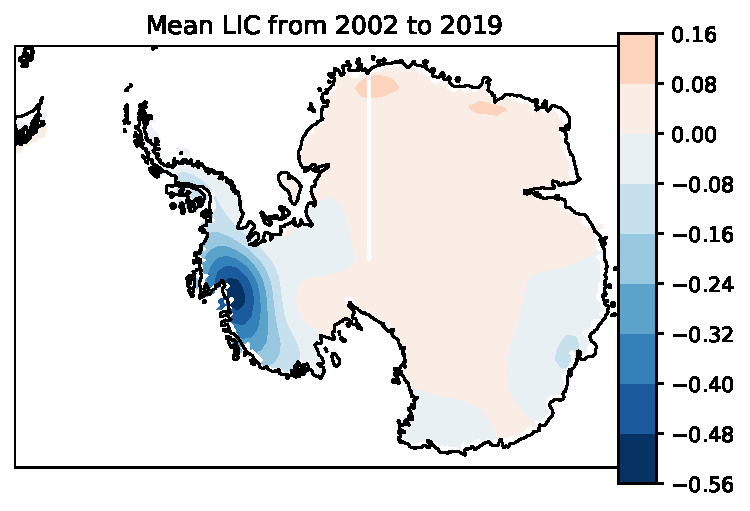
\includegraphics{images/2021w4/mean_spatial_plots2/hres/LIC}
     \caption{Mean value of \gls{lilwet} from 2002 to 2017.}
     \label{fig:lilwet_mean}
 \end{figure}
 
\textcolor{red}{Plot of mean time-series of Antarctic ice}\\
\begin{figure}[H]
    \centering
    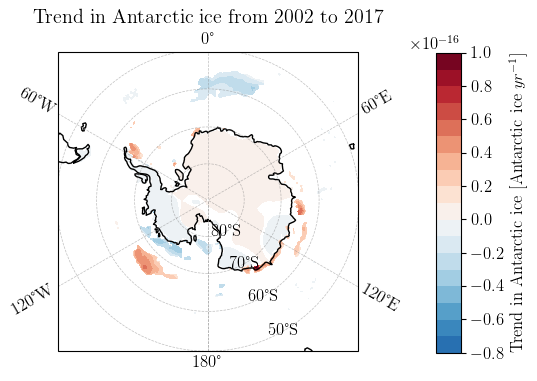
\includegraphics{images/2021w5/chapter7/lres/trend_spatial_ICE.png}
    \caption{Caption}
    \label{fig:my_label}
\end{figure}

The simplest thing we can do at this point is to compare the mean time series of this with different variables.

\section{Comparing land ice with different variables}
For the first step in analysis here we plotted the mean values for both land ice and other environmental variables, considering only the grid points where we have data for land ice.

\subsection{Trends in different variables}
\textcolor{red}{Plot of trend in Temperature, subsurface temperature, ozone, precipitation, wind speed}

\subsection{Visual time series comparison}

\subsection{Co-spatial Correlations}

\section{Identifying drivers for significant decrease}

\subsection{Identifying region with significant decrease}

\subsection{Spatial correlations}

\subsection{Regressions}

\section{Discussion and implications of these results}

\end{document}